%% bare_jrnl.tex
%% V1.3
%% 2007/01/11
%% by Michael Shell
%% see http://www.michaelshell.org/
%% for current contact information.
%%
%% This is a skeleton file demonstrating the use of IEEEtran.cls
%% (requires IEEEtran.cls version 1.7 or later) with an IEEE journal paper.
%%
%% Support sites:
%% http://www.michaelshell.org/tex/ieeetran/
%% http://www.ctan.org/tex-archive/macros/latex/contrib/IEEEtran/
%% and
%% http://www.ieee.org/



% *** Authors should verify (and, if needed, correct) their LaTeX system  ***
% *** with the testflow diagnostic prior to trusting their LaTeX platform ***
% *** with production work. IEEE's font choices can trigger bugs that do  ***
% *** not appear when using other class files.                            ***
% The testflow support page is at:
% http://www.michaelshell.org/tex/testflow/


%%*************************************************************************
%% Legal Notice:
%% This code is offered as-is without any warranty either expressed or
%% implied; without even the implied warranty of MERCHANTABILITY or
%% FITNESS FOR A PARTICULAR PURPOSE! 
%% User assumes all risk.
%% In no event shall IEEE or any contributor to this code be liable for
%% any damages or losses, including, but not limited to, incidental,
%% consequential, or any other damages, resulting from the use or misuse
%% of any information contained here.
%%
%% All comments are the opinions of their respective authors and are not
%% necessarily endorsed by the IEEE.
%%
%% This work is distributed under the LaTeX Project Public License (LPPL)
%% ( http://www.latex-project.org/ ) version 1.3, and may be freely used,
%% distributed and modified. A copy of the LPPL, version 1.3, is included
%% in the base LaTeX documentation of all distributions of LaTeX released
%% 2003/12/01 or later.
%% Retain all contribution notices and credits.
%% ** Modified files should be clearly indicated as such, including  **
%% ** renaming them and changing author support contact information. **
%%
%% File list of work: IEEEtran.cls, IEEEtran_HOWTO.pdf, bare_adv.tex,
%%                    bare_conf.tex, bare_jrnl.tex, bare_jrnl_compsoc.tex
%%*************************************************************************

% Note that the a4paper option is mainly intended so that authors in
% countries using A4 can easily print to A4 and see how their papers will
% look in print - the typesetting of the document will not typically be
% affected with changes in paper size (but the bottom and side margins will).
% Use the testflow package mentioned above to verify correct handling of
% both paper sizes by the user's LaTeX system.
%
% Also note that the "draftcls" or "draftclsnofoot", not "draft", option
% should be used if it is desired that the figures are to be displayed in
% draft mode.
%
\documentclass[journal,twocolumn]{IEEEtran}
%
% If IEEEtran.cls has not been installed into the LaTeX system files,
% manually specify the path to it like:
% \documentclass[journal]{../sty/IEEEtran}





% Some very useful LaTeX packages include:
% (uncomment the ones you want to load)


% *** MISC UTILITY PACKAGES ***
%
%\usepackage{ifpdf}
% Heiko Oberdiek's ifpdf.sty is very useful if you need conditional
% compilation based on whether the output is pdf or dvi.
% usage:
% \ifpdf
%   % pdf code
% \else
%   % dvi code
% \fi
% The latest version of ifpdf.sty can be obtained from:
% http://www.ctan.org/tex-archive/macros/latex/contrib/oberdiek/
% Also, note that IEEEtran.cls V1.7 and later provides a builtin
% \ifCLASSINFOpdf conditional that works the same way.
% When switching from latex to pdflatex and vice-versa, the compiler may
% have to be run twice to clear warning/error messages.






% *** CITATION PACKAGES ***
%
%\usepackage{cite}
% cite.sty was written by Donald Arseneau
% V1.6 and later of IEEEtran pre-defines the format of the cite.sty package
% \cite{} output to follow that of IEEE. Loading the cite package will
% result in citation numbers being automatically sorted and properly
% "compressed/ranged". e.g., [1], [9], [2], [7], [5], [6] without using
% cite.sty will become [1], [2], [5]--[7], [9] using cite.sty. cite.sty's
% \cite will automatically add leading space, if needed. Use cite.sty's
% noadjust option (cite.sty V3.8 and later) if you want to turn this off.
% cite.sty is already installed on most LaTeX systems. Be sure and use
% version 4.0 (2003-05-27) and later if using hyperref.sty. cite.sty does
% not currently provide for hyperlinked citations.
% The latest version can be obtained at:
% http://www.ctan.org/tex-archive/macros/latex/contrib/cite/
% The documentation is contained in the cite.sty file itself.






% *** GRAPHICS RELATED PACKAGES ***
%
\ifCLASSINFOpdf
  % \usepackage[pdftex]{graphicx}
  % declare the path(s) where your graphic files are
  % \graphicspath{{../pdf/}{../jpeg/}}
  % and their extensions so you won't have to specify these with
  % every instance of \includegraphics
  % \DeclareGraphicsExtensions{.pdf,.jpeg,.png}
\else
  % or other class option (dvipsone, dvipdf, if not using dvips). graphicx
  % will default to the driver specified in the system graphics.cfg if no
  % driver is specified.
  % \usepackage[dvips]{graphicx}
  % declare the path(s) where your graphic files are
  % \graphicspath{{../eps/}}
  % and their extensions so you won't have to specify these with
  % every instance of \includegraphics
  % \DeclareGraphicsExtensions{.eps}
\fi
% graphicx was written by David Carlisle and Sebastian Rahtz. It is
% required if you want graphics, photos, etc. graphicx.sty is already
% installed on most LaTeX systems. The latest version and documentation can
% be obtained at: 
% http://www.ctan.org/tex-archive/macros/latex/required/graphics/
% Another good source of documentation is "Using Imported Graphics in
% LaTeX2e" by Keith Reckdahl which can be found as epslatex.ps or
% epslatex.pdf at: http://www.ctan.org/tex-archive/info/
%
% latex, and pdflatex in dvi mode, support graphics in encapsulated
% postscript (.eps) format. pdflatex in pdf mode supports graphics
% in .pdf, .jpeg, .png and .mps (metapost) formats. Users should ensure
% that all non-photo figures use a vector format (.eps, .pdf, .mps) and
% not a bitmapped formats (.jpeg, .png). IEEE frowns on bitmapped formats
% which can result in "jaggedy"/blurry rendering of lines and letters as
% well as large increases in file sizes.
%
% You can find documentation about the pdfTeX application at:
% http://www.tug.org/applications/pdftex





% *** MATH PACKAGES ***
%
%\usepackage[cmex10]{amsmath}
% A popular package from the American Mathematical Society that provides
% many useful and powerful commands for dealing with mathematics. If using
% it, be sure to load this package with the cmex10 option to ensure that
% only type 1 fonts will utilized at all point sizes. Without this option,
% it is possible that some math symbols, particularly those within
% footnotes, will be rendered in bitmap form which will result in a
% document that can not be IEEE Xplore compliant!
%
% Also, note that the amsmath package sets \interdisplaylinepenalty to 10000
% thus preventing page breaks from occurring within multiline equations. Use:
%\interdisplaylinepenalty=2500
% after loading amsmath to restore such page breaks as IEEEtran.cls normally
% does. amsmath.sty is already installed on most LaTeX systems. The latest
% version and documentation can be obtained at:
% http://www.ctan.org/tex-archive/macros/latex/required/amslatex/math/





% *** SPECIALIZED LIST PACKAGES ***
%
%\usepackage{algorithmic}
% algorithmic.sty was written by Peter Williams and Rogerio Brito.
% This package provides an algorithmic environment fo describing algorithms.
% You can use the algorithmic environment in-text or within a figure
% environment to provide for a floating algorithm. Do NOT use the algorithm
% floating environment provided by algorithm.sty (by the same authors) or
% algorithm2e.sty (by Christophe Fiorio) as IEEE does not use dedicated
% algorithm float types and packages that provide these will not provide
% correct IEEE style captions. The latest version and documentation of
% algorithmic.sty can be obtained at:
% http://www.ctan.org/tex-archive/macros/latex/contrib/algorithms/
% There is also a support site at:
% http://algorithms.berlios.de/index.html
% Also of interest may be the (relatively newer and more customizable)
% algorithmicx.sty package by Szasz Janos:
% http://www.ctan.org/tex-archive/macros/latex/contrib/algorithmicx/




% *** ALIGNMENT PACKAGES ***
%
%\usepackage{array}
% Frank Mittelbach's and David Carlisle's array.sty patches and improves
% the standard LaTeX2e array and tabular environments to provide better
% appearance and additional user controls. As the default LaTeX2e table
% generation code is lacking to the point of almost being broken with
% respect to the quality of the end results, all users are strongly
% advised to use an enhanced (at the very least that provided by array.sty)
% set of table tools. array.sty is already installed on most systems. The
% latest version and documentation can be obtained at:
% http://www.ctan.org/tex-archive/macros/latex/required/tools/


%\usepackage{mdwmath}
%\usepackage{mdwtab}
% Also highly recommended is Mark Wooding's extremely powerful MDW tools,
% especially mdwmath.sty and mdwtab.sty which are used to format equations
% and tables, respectively. The MDWtools set is already installed on most
% LaTeX systems. The lastest version and documentation is available at:
% http://www.ctan.org/tex-archive/macros/latex/contrib/mdwtools/


% IEEEtran contains the IEEEeqnarray family of commands that can be used to
% generate multiline equations as well as matrices, tables, etc., of high
% quality.


%\usepackage{eqparbox}
% Also of notable interest is Scott Pakin's eqparbox package for creating
% (automatically sized) equal width boxes - aka "natural width parboxes".
% Available at:
% http://www.ctan.org/tex-archive/macros/latex/contrib/eqparbox/





% *** SUBFIGURE PACKAGES ***
%\usepackage[tight,footnotesize]{subfigure}
% subfigure.sty was written by Steven Douglas Cochran. This package makes it
% easy to put subfigures in your figures. e.g., "Figure 1a and 1b". For IEEE
% work, it is a good idea to load it with the tight package option to reduce
% the amount of white space around the subfigures. subfigure.sty is already
% installed on most LaTeX systems. The latest version and documentation can
% be obtained at:
% http://www.ctan.org/tex-archive/obsolete/macros/latex/contrib/subfigure/
% subfigure.sty has been superceeded by subfig.sty.



%\usepackage[caption=false]{caption}
%\usepackage[font=footnotesize]{subfig}
% subfig.sty, also written by Steven Douglas Cochran, is the modern
% replacement for subfigure.sty. However, subfig.sty requires and
% automatically loads Axel Sommerfeldt's caption.sty which will override
% IEEEtran.cls handling of captions and this will result in nonIEEE style
% figure/table captions. To prevent this problem, be sure and preload
% caption.sty with its "caption=false" package option. This is will preserve
% IEEEtran.cls handing of captions. Version 1.3 (2005/06/28) and later 
% (recommended due to many improvements over 1.2) of subfig.sty supports
% the caption=false option directly:
%\usepackage[caption=false,font=footnotesize]{subfig}
%
% The latest version and documentation can be obtained at:
% http://www.ctan.org/tex-archive/macros/latex/contrib/subfig/
% The latest version and documentation of caption.sty can be obtained at:
% http://www.ctan.org/tex-archive/macros/latex/contrib/caption/




% *** FLOAT PACKAGES ***
%
%\usepackage{fixltx2e}
% fixltx2e, the successor to the earlier fix2col.sty, was written by
% Frank Mittelbach and David Carlisle. This package corrects a few problems
% in the LaTeX2e kernel, the most notable of which is that in current
% LaTeX2e releases, the ordering of single and double column floats is not
% guaranteed to be preserved. Thus, an unpatched LaTeX2e can allow a
% single column figure to be placed prior to an earlier double column
% figure. The latest version and documentation can be found at:
% http://www.ctan.org/tex-archive/macros/latex/base/



%\usepackage{stfloats}
% stfloats.sty was written by Sigitas Tolusis. This package gives LaTeX2e
% the ability to do double column floats at the bottom of the page as well
% as the top. (e.g., "\begin{figure*}[!b]" is not normally possible in
% LaTeX2e). It also provides a command:
%\fnbelowfloat
% to enable the placement of footnotes below bottom floats (the standard
% LaTeX2e kernel puts them above bottom floats). This is an invasive package
% which rewrites many portions of the LaTeX2e float routines. It may not work
% with other packages that modify the LaTeX2e float routines. The latest
% version and documentation can be obtained at:
% http://www.ctan.org/tex-archive/macros/latex/contrib/sttools/
% Documentation is contained in the stfloats.sty comments as well as in the
% presfull.pdf file. Do not use the stfloats baselinefloat ability as IEEE
% does not allow \baselineskip to stretch. Authors submitting work to the
% IEEE should note that IEEE rarely uses double column equations and
% that authors should try to avoid such use. Do not be tempted to use the
% cuted.sty or midfloat.sty packages (also by Sigitas Tolusis) as IEEE does
% not format its papers in such ways.


%\ifCLASSOPTIONcaptionsoff
%  \usepackage[nomarkers]{endfloat}
% \let\MYoriglatexcaption\caption
% \renewcommand{\caption}[2][\relax]{\MYoriglatexcaption[#2]{#2}}
%\fi
% endfloat.sty was written by James Darrell McCauley and Jeff Goldberg.
% This package may be useful when used in conjunction with IEEEtran.cls'
% captionsoff option. Some IEEE journals/societies require that submissions
% have lists of figures/tables at the end of the paper and that
% figures/tables without any captions are placed on a page by themselves at
% the end of the document. If needed, the draftcls IEEEtran class option or
% \CLASSINPUTbaselinestretch interface can be used to increase the line
% spacing as well. Be sure and use the nomarkers option of endfloat to
% prevent endfloat from "marking" where the figures would have been placed
% in the text. The two hack lines of code above are a slight modification of
% that suggested by in the endfloat docs (section 8.3.1) to ensure that
% the full captions always appear in the list of figures/tables - even if
% the user used the short optional argument of \caption[]{}.
% IEEE papers do not typically make use of \caption[]'s optional argument,
% so this should not be an issue. A similar trick can be used to disable
% captions of packages such as subfig.sty that lack options to turn off
% the subcaptions:
% For subfig.sty:
% \let\MYorigsubfloat\subfloat
% \renewcommand{\subfloat}[2][\relax]{\MYorigsubfloat[]{#2}}
% For subfigure.sty:
% \let\MYorigsubfigure\subfigure
% \renewcommand{\subfigure}[2][\relax]{\MYorigsubfigure[]{#2}}
% However, the above trick will not work if both optional arguments of
% the \subfloat/subfig command are used. Furthermore, there needs to be a
% description of each subfigure *somewhere* and endfloat does not add
% subfigure captions to its list of figures. Thus, the best approach is to
% avoid the use of subfigure captions (many IEEE journals avoid them anyway)
% and instead reference/explain all the subfigures within the main caption.
% The latest version of endfloat.sty and its documentation can obtained at:
% http://www.ctan.org/tex-archive/macros/latex/contrib/endfloat/
%
% The IEEEtran \ifCLASSOPTIONcaptionsoff conditional can also be used
% later in the document, say, to conditionally put the References on a 
% page by themselves.





% *** PDF, URL AND HYPERLINK PACKAGES ***
%
%\usepackage{url}
% url.sty was written by Donald Arseneau. It provides better support for
% handling and breaking URLs. url.sty is already installed on most LaTeX
% systems. The latest version can be obtained at:
% http://www.ctan.org/tex-archive/macros/latex/contrib/misc/
% Read the url.sty source comments for usage information. Basically,
% \url{my_url_here}.





% *** Do not adjust lengths that control margins, column widths, etc. ***
% *** Do not use packages that alter fonts (such as pslatex).         ***
% There should be no need to do such things with IEEEtran.cls V1.6 and later.
% (Unless specifically asked to do so by the journal or conference you plan
% to submit to, of course. )


% correct bad hyphenation here
\hyphenation{op-tical net-works semi-conduc-tor}

%% load necessary packages
% \documentclass[paper=a4, fontsize=10pt,headings=small]{scrartcl}
% \documentclass[paper=a4, fontsize=10pt,headings=small]{scrartcl}
% \documentclass[journal,onecolumn]{IEEEtran}
% \documentclass[paper=a4, fontsize=10pt,parskip=half,headings=small]{scrartcl}
\usepackage{check-short}
\usepackage{overpic}
\usepackage{multirow}


%% set author information etc
\title{Why perfusion measurements will fail}
\author{Constantin Sandmann, Erik A. Hanson, Alexander Malyshev,  Arvid Lundervold, Jan Modersitzki, Erlend Hodneland }
\date{\today}


%% define some local commands
\newcommand{\Qso}{Q_{\mathrm{so}}}
\newcommand{\Qsi}{Q_{\mathrm{si}}}
\newcommand{\ca}{c_\mathrm{a}}
\newcommand{\CBV}{\mathrm{CBV}}
\newcommand{\MTT}{\mathrm{MTT}}
\newcommand{\cout}{c_{\mathrm{v}}}
\newcommand{\Pa}{P_{\mathrm{a}}}
\newcommand{\Pout}{P_{\mathrm{v}}}
\newcommand{\Perf}{P}
\newcommand{\Perfv}{P_{\mathrm{v}}}
\newcommand{\Perfs}{P_{\mathrm{s}}}
\newcommand{\Flow}{F}

%define SI-units, since we want to be able to easily change them
% \newcommand{\simu}{k\pascal$\cdot$\second} %CH: I have problems compiling with the cdot
\newcommand{\simu}{k\pascal\second}
\newcommand{\siFmm}{\milli\meter\cubed\per\second}
\newcommand{\siFml}{\milli\litre\per\second}
\newcommand{\siQmm}{\milli\meter\cubed\per\second\per\milli\meter\cubed}
\newcommand{\siPml}{\milli\litre\per\minute\per100\milli\litre}
\newcommand{\siq}{\milli\meter\cubed\per\second\per\milli\meter\squared}
\newcommand{\siml}{\milli\litre}
\newcommand{\siphimm}{\milli\meter\cubed\per\milli\meter\cubed}
\newcommand{\siJ}{\milli\mol\per\second\per\milli\meter\squared}
\newcommand{\siphi}{\milli\meter\cubed\per\milli\meter\cubed}
\newcommand{\sirho}{\milli\gram\per\milli\meter\cubed}
\newcommand{\siQtilde}{\milli\gram\per\second\per\milli\meter\cubed}
\newcommand{\sic}{\milli\mol\per\milli\meter\cubed}
\newcommand{\simm}{\milli\meter\cubed}

%\newcommand{\siP}{\cubic\milli\meter\per\second\per\cubic\milli\meter}
%\newcommand{\siP}{\milli\meter\cubed\per\second}
%\newcommand{\siPml}{\milli\litre\per\second}
%\newcommand{\siQtilde}{\milli\gram\per\second\per\milli\meter\cubed}
%\newcommand{\siQ}{\milli\meter\cubed\per\second\per\milli\meter\cubed}
%\newcommand{\sirho}{\milli\gram\per\milli\meter\cubed}
%\newcommand{\sic}{\milli\mol\per\milli\meter\cubed}
%\newcommand{\siPn}{\milli\litre\per\minute\per100\milli\litre}
%\newcommand{\simm}{\milli\meter\cubed}


%define misc commands
\newcommand{\missingsource}{\textcolor{red}{[?]}}
\newlength{\fwd}

%--------------------------------------------------------------------------------------------
%--------------------------------------------------------------------------------------------
% Here begins the document, remove "draft" option in document class to include images
%--------------------------------------------------------------------------------------------
%--------------------------------------------------------------------------------------------
\begin{document}
	%--------------------------------------------------
	% Title Page=
	%--------------------------------------------------
	\maketitle
%	\tableofcontents

	\begin{abstract}
		In perfusion imaging the usage of traditional one-compartment models to estimate hemodynamic parameters like blood flow (perfusion), blood volume and mean transit times is widespread. In this paper we show limits of traditional models to recover perfusion in coupled systems. Based on modeling of porous media flow, we introduce a continuous model for propagation of a tracer in the capillary tissue. We show that the proposed model can be understood as a coupled set of traditional one-compartment models. It is furthermore demonstrated that traditional models (deconvolution, maximum slope) are accurately recovering the perfusion if applied to the full system. However, it is shown both analytically and experimentally that results of traditional models are not meaningful if applied only to smaller portions of the system, and will result in overestimation of perfusion. Evidence of real patient data is provided, indicating that this effect might also be observed in real-life applications.  As a remedy, we propose to define perfusion mathematically in coupled systems as laminar flow along the streamlines.
	\end{abstract}

	%--------------------------------------------------
	%--------------------------------------------------
	% Section: Introduction
	%--------------------------------------------------
	%--------------------------------------------------
	\section{Introduction}
	
	Quantitative measurements of hemodynamic medical parameters based on tracer kinetic modeling are widespread both in research and in clinical practice \cite{sourbron13}. 
	In the present work, we focus on mathematical models to estimate blood perfusion (cerebral blood flow, CBF), blood volume (cerebral blood volume, CBV), and mean transit time (MTT) of the brain from contrast-enhanced dynamic image data. 

	While hardware limitations in medical imaging for decades have confined studies to only handle larger tissue regions or full organs, modern imaging technology and voxel based analysis give rise to aspirations about detailed perfusion maps with sub-millimeter precision.  
	Examples of estimated parameter maps are found in i.e. \cite{Feng2013,Chen2011}. 
	Quantitative perfusion maps, as well as other parameter maps arising from tracer kinetic modeling, can be combined with anatomical information, and the maps have proven to be of particular value in e.g. stroke studies for localization of trauma. 
	Among the physiological parameters obtainable from tracer kinetic models, CBF has proven to be particularly difficult to reliably describe on a voxel-basis \cite{kudo10}.
	Causes for these limitations in perfusion estimations are issues in the numerical implementation \cite{kudo10}, but might also depend on over-simplified dynamic models, which were originally designed to describe larger volumes of interest \cite{zierler00}.	
 	Even though voxel wise perfusion measurements are difficult to establish, examples of perfusion maps are extensively reported in the literature \cite{Feng2013,Chen2011}.
	
	There have been several approaches to clarify the concept of perfusion in a continuous sense.
	In \cite{calamante03}, dispersion of the arterial input function was simulated using Navier-Stokes equations.
	It was shown that neglecting to account for dispersion can have adverse impact on perfusion measurements.
	More recently, a mathematical theory for voxelwise perfusion was introduced in \cite{sourbron14} as an alternative to the traditional region of interest (ROI) based models.
	However, evaluation of the proposed modeling is still pending.
	
	In this work we focus on the validity of traditional perfusion models.
	% Specifically, we demonstrate one approach for interpretation of tradition perfusion models, as if they were obtained from a coupled system where one volume is feeding the direct neighbors.
	We do this by simulating a tissue patch with one inlet, one outlet, and a highly developed capillary system in between.
	A directional flow field for the patch is set up according to Darcy's law from porous media flow \cite{Darcy56}, assuming that blood flow is mainly driven by pressure differences.	
	After that, contrast agent propagation in this patch is simulated using standard transport equations.%, cf. Section~\ref{sec:transport}.
	% Details on the simulation can be found in Section~\ref{sec:synthetic}.	
	As a result, we show that the resulting 3D system can be equivalently described by a coupled set of multiple traditional one-compartment models, in line with the physical environment where each control volume is feeding the direct neighbors.

	We then proceed to demonstrate that traditional models like deconvolution or maximum slope are able to recover the perfusion accurately if applied to the whole system.
	However, when applying the traditional models to isolated parts of the full system, we find that local perfusion in coupled systems is not straight-forward to define.
	In order to cope with this issue, two possible definitions of voxel-wise perfusion are presented: A definition $\Perfv$ which is closely connected to the concept of local arterial input functions and a tailored definition for continuous models $\Perfs$.
	
	Our results show that perfusion results from traditional models tend to overestimate $\Perfs$ and to underestimate $\Perfv$ if they are applied only to parts of the full system.
	% In Section~\ref{sec:NewAndOld} 
	Analytic results are given, which show that the recovered perfusion depends on all upstream flow and not only on the local value.
	%In Section~\ref{sec:RealData} we 
	We also show results indicating that overestimation of perfusion due to coupling might also be found in real data.
	
In light of expected improvements in spatial resolution of medical scanners, traditional models will increasingly fail to accurately measure blood-flow when applied to patches of the capillary system. Instead, this establishes the need for continuous models as e.g. proposed in \cite{sourbron14}.
	% We will further elaborate on the implications of this in Section~\ref{sec:conclusion}.
	
	
	%--------------------------------------------------
	%--------------------------------------------------
	% Section: Traditional models
	%--------------------------------------------------
	%--------------------------------------------------
	\section{Traditional Models for perfusion} \label{sec:traditional}

	In this section we describe  the convolution- and the maximum slope model, two widely used one-compartment pharmacokinetic models for measurements of CBF and CBV. These models were chosen for investigating the behaviour of traditional indicator dilution theory at finer scales. For the remaining, they are referred to as \emph{traditional} models.
	%We will start by presenting the continuity equation for tracer kinetic modeling \eqref{eq:classicgeneral} which is basic to most models for CBF estimation.
	%To simplify the very general model \eqref{eq:classicgeneral}, we will then present two different additional assumptions, which lead to the most common models for CBF estimation: Namely the maximum slope model and the deconvolution model.
	%Note that an excellent and more detailed coverage of the proposed models can be found in \cite{sourbron13,klotz99}.
	
	Let $\Omega_i$ be an arbitrary control volume with one inlet and one outlet, and let $C(t)$ denote the average contrast agent (CA) concentration within $\Omega_i$ at timepoint $t$.
	The traditional model assumes that the change of concentration at timepoint $t$ can be described by the ordinary differential equation $C'(t) = \Pa\ca(t) - \Pout\cout(t)$. 
	Here $\ca,\cout$ are the CA plasma concentrations at the inlet and outlet of $\Omega_i$, and $\Pa,\Pout$ are the corresponding perfusion values at these locations.
	Assuming incompressible flow leads to $\Pa = \Pout$ and hence we obtain the general form
	\begin{equation}
		C'(t) = \Pa\left(\ca(t) - \cout(t)\right).
		\label{eq:classicgeneral}
	\end{equation}	
	In the following it is assumed that the plasma tracer concentration $\ca$ at the inlet is known.
	In clinical practice this can be implemented by measuring $\ca$ directly in a feeding artery \cite{ostergaard96}.
	%However, note that if different volumes of interest are feeding each other, this assumption might not be correct and might lead to errors in the recovered flow.
	% We will elaborate on consequences of this in Section~\ref{sec:NewAndOld} and Section~\ref{sec:synthetic}.
	Since $\cout$ is usually unknown, additional assumptions need to be made if one wants to reconstruct $\Pa$ from a given tissue curve $C$. The convolution model and the maximum slope (MS) model diverge in further assumptions.
	
	

	%----------------------------------------------------------
	% Subsection: The Convolution Model: Theory and Implementation
	%----------------------------------------------------------	
	\subsection{The Convolution Model}\label{sec:conv}
	
	For the deconvolution model, one approach is to assume there is an unknown probability distribution of transit times $h$ through $\Omega_i$. 
	This leads to
	\begin{equation}
		\cout(t) = (h*\ca)(t) := \int_0^t \ca(s) h(t-s) \diffint s.
	\end{equation}
	Combining this with \eqref{eq:classicgeneral} yields $C'(t) = \Pa\ca(t)-\Pa (h*\ca)(t)$.
	Integrating this equation and using basic properties of the convolution one obtains the general solution
	\begin{equation}
		C(t) = (I*\ca)(t).
		\label{eq:conv}
	\end{equation}
	where the \emph{impuls-response function} $I$ is defined as $I(t) := \Pa(1-\int_0^t h(s) \diffint s)$.
	The task of identifying $I(t)$ given a tissue curve $C(t)$ and an arterial input function $\ca(t)$ is a deconvolution problem.
	If $I(t)$ is recovered, $\Pa$ can subsequently be estimated as $\Pa = \max_{t} I(t)$.
	There are several methods to perform the deconvolution.
	A standard approach using Fourier-based algorithms is sensitive to the presence of noise \cite{ostergaard96}.
	Another class of deconvolution algorithms gaining increasing attention are based on Bayesian modeling \cite{boutelier12}.
	However the numerical handling is still difficult since complex and error-prone numerical integration has to be performed \cite{boutelier12}.
	A popular class among deconvolution algorithms is based on singular value decomposition (SVD) \cite{ostergaard96}.
	These algorithms have shown to be robust for a reasonable noise level.
	Also, they can be easily adapted to be robust against delays in tracer arrival using block-circular structures (bSVD cf. \cite{wu03}).
	In order to identify the impuls-response function $I(t)$ from simulated data, we hence decided to use the bSVD model as proposed in \cite{wu03}.

	%----------------------------------------------------------
	% Subsection: A Second Digital Phantom For Validation
	%----------------------------------------------------------	
%	\subsection{The Convolution Model for a Well-Mixed Compartment \textcolor{red}{Haven't we used this assumption earlier?}} \label{sec:comp}

% Now, let $\phi$ be the porosity of the tissue, which is the relative distribution volume of the blood. Both CBV and $\phi$ describe the relative motile fluid volume of a control volume, and they are therefore essentially equal. For simplicity we will use the short form notation $\phi$ in the mathematical arguments following.   If we make the assumption of $\Omega_i$ as a well-mixed compartment where $C(t) = \phi\cout(t)$ for a porosity $0 \le \phi \le 1$, \eqref{eq:classicgeneral} reduces to the initial value problem
% 	\begin{align}
% 		(\phi \cout)' &= \Pa \ca - \Pa \cout, \nonumber \\
% 		\cout(0)&=0,
% 		\label{eq:dcdt}
% 	\end{align}
% 	where we also assume no tracer within the compartment for $t = 0$.
% 	Denote the mean transit time $T:=\Pa/ \phi$ for $\phi \ne 0$, and \eqref{eq:dcdt} yields the solution of $c_v$, leading to the traditional perfusion model
% 	\begin{equation}
% 		C(t) = \Pa \int_0^t e^{-(t-s)/T}\ca(s)\diffint s
% 		\label{eq:traditionalperf}
% 	\end{equation}
% 	with the impulse response function $I(t)=\Pa e^{-t/T}$.

	
	
	
	%----------------------------------------------------------
	% Subsection: The Maximum Slope Model
	%----------------------------------------------------------
	\subsection{The Maximum Slope Model}\label{sec:ms}	
	In the MS model it is assumed that when $\ca$ has its maximum, only a negligible amount of CA is leaving the system \cite{klotz99}.
	For this time interval, \eqref{eq:classicgeneral} reduces to 
	\begin{equation}
		C'(t) = \Pa\ca(t),
	\end{equation}
	in case one can see that if $\ca$ has a maximum, also $C'$ must have a maximum since stationarity in $\Pa$ is assumed.
	Hence, it holds that
	\begin{equation}\label{eq:MS}
		\Pa = \frac{\max_{t}C'(t)}{\max_{t}\ca(t)}.
	\end{equation}
	
	
	
	%--------------------------------------------------
	%--------------------------------------------------
	% Section: The synthetic model
	%--------------------------------------------------
	%--------------------------------------------------	
	\section{A Synthetic Model for Capillary Flow}\label{sec:synthetic}
	
	% Structurally, the assumptions for the convolution model as well as the maximum slope model presented in Section \ref{sec:traditional} are similar.
	The validity of the traditional methods rely on a ROI with only one inlet and one outlet, and that transition times are prescribed by some probability distribution.
	In fact, the assumption of one inlet and one outlet  may easily be violated when we locally describe CA propagation through a larger volume with a highly developed capillary system.
	For this type of model system we instead expect a set of coupled transport equations where each voxel can be regarded as an inlet for surrounding voxels.
	Hence, in order to make a realistic synthetic model for capillary flow, we decided to describe the CA propagation as a spatially coupled transport process, i.e. using partial differential equations (PDE) for transport. This PDE model is used for validation of the traditional models. 
	
	%We start by introducing the modeling of a directional flow field in the simulated patch in Section~\ref{sec:flow}.
	Compatible with the assumption of stationary, incompressible flow at low Reynold numbers within the capillary system \cite{Cho2011}, we will use Darcy's law to simulate capillary flow \cite{Darcy56}. This is in agreement with previous work on capillary perfusion \cite{Cookson2012,Michler2013}. 
	% For simplicity, we also assume an isotropic porous media.
	% Additional parameters represented in the model were blood viscosity and a possibly anisotropic permeability.
	% However, for sake of argument permeability was assumed to be isotropic and constant.
	A major difference between our coupled flow model and traditional tracer kinetic modeling is the normalization of the flow field within the traditional models,
using volume normalized fluid flow with units [\si{\siQmm}], referred to as perfusion, as a quantity to describe fluid transport. 
	% However, we will show in Section~\ref{sec:flux2perf} that the concept of perfusion is discretization dependent. 
	However, to avoid a discretization dependent flow field, for the PDE model we instead use vector valued surface fluid flux $q = q(x)$ with units [\si{\siq}], in agreement with geoscience and porous media simulation theory.
	The fluid flux is a vector field describing the volume of fluid per unit time flowing across a sliced unit area of the sample.	
	% A model to convert vector valued flux to scalar valued perfusion with units [\si{\siQmm}] will be introduced in Section \ref{sec:flux2perf}.
	Apart from the normalization with respect to surface, the assumptions of linearity and stationarity in the fluid flux are in complete agreement with standard pharmacokinetic modeling \cite{sourbron13}.
	
	%Having obtained a 3D directional flow field, we proceed to simulate contrast agent propagation proportional to the flow using linear transport equations, cf. Section~\ref{sec:traditional}.
	%In the modeling of the transport we account for fractional blood volume as well as conservation of contrast agent mass.
	%Since we assume that contrast agent propagates along the capillaries, we decided to neglect effects by diffusion.
	%Note that modeling of the transport is in line with standard porous media theory \cite{Aarnes2007}.
	
	
	

	
	%--------------------------------------------------
	% Subsection: Modeling the Blood Flow
	%--------------------------------------------------
	\subsection{Modelling Capillary Blood Flow}\label{sec:flow}
	
	%We will here set up a framework for modeling the blood flow as a fluid flow through a porous medium. 
	For the time being we will not consider contrast agent concentrations, but only the fluid flow in general.
	The fluid density is denoted by $\rho = \rho(x,t)$. 
	% [\si{\sirho}].
	The flux $q$ as well as the porosity 
	% $\phi$ [\si{\simm}/\si{\simm}] 
	are assumed to be stationary and hence independent of time.
	Fluid entering and leaving the system is described by a source- and sink term $\tilde{Q} = \tilde{Q}(x)$ [\si{\siQtilde}]. 
	The continuity equation describing conservation of fluid mass states
	\begin{equation}
		\frac{\partial (\phi \rho)}{\partial t} + \nabla \cdot (\rho q) = \tilde{Q}.
		\label{eq:syntcont}
	\end{equation} 
	Furthermore, assuming that the fluid flow is steady-state and that the density of blood $\rho$ is constant in space, we obtain $\nabla \cdot q = \tilde{Q}/\rho$.
	In order to scale away the density $\rho$ we define $Q$ [\si{\siQmm}] having the relation $\tilde{Q} := Q\rho$, thus transforming the equation into 
	\begin{equation}
		\nabla \cdot q = Q
		\label{eq:syntcontsimp}
	\end{equation}
	where the right hand side is a volume flux, only non-zero within the source or the sink. 
	Elsewhere, \eqref{eq:syntcontsimp} is concurrent with divergence free flow of an incompressible fluid.
	
	Low velocity fluid flux in porous media is usually described by Darcy's law. Neglecting gravitational forces leads to \cite{Darcy56}
	\begin{equation}
		q = -\frac{\mathbf{k}}{\mu} \nabla p.
		\label{eq:syntdarcysimp}
	\end{equation}
	Here, $\mathbf{k} = \mathbf{k}(x)$ is the permeability tensor, $p=p(x)$ is the pressure, and $\mu = \mu(x)$ is the viscosity of the fluid. 	
	For simplicity, we will assume that $\mathbf{k}$ is a symmetric and positive definite tensor with only nonzero diagonal elements $\mathbf{k}_{ii} = k$, in accordance with a homogeneous porous medium.	
	Equations \eqref{eq:syntcontsimp} and \eqref{eq:syntdarcysimp} can be combined, yielding the following elliptic partial differential equation in the pressure-field $p$ within the closed domain $\Omega$,
	\begin{equation}
		\left\vert
		\begin{alignedat}{2}
			\nabla \cdot \left( -\frac{\mathbf{k}}{\mu} \nabla p \right) &= Q  \qquad &&x \in \Omega, \\
			n \cdot \nabla p &=0 &&x \in \partial \Omega
		\end{alignedat}
		\right\vert 
		\label{eq:flowmodel}
	\end{equation}
	where we also added Neuman boundary conditions reflecting zero fluid flux $q(x)$ across $\partial \Omega$.
	Here, $\partial \Omega$ denotes the boundary of $\Omega$ and $n$ the outward unit normal vector. 
	Note that \eqref{eq:flowmodel} defines a solution which is only unique up to constant \cite{evans98}.
	After solving \eqref{eq:flowmodel} for the pressure $p$, the flux field can be computed according to \eqref{eq:syntdarcysimp} from the obtained pressure map. 
	
	

	
	
	
			
	%--------------------------------------------------
	% Subsection: Modeling the Contrast Agent Transport
	%--------------------------------------------------	
	\subsection{Modelling Indicator Dilution}\label{sec:transport}

	%In Section \ref{sec:flow} we introduced a model describing blood flow through fluxes and pressure fields. 
	The introduced framework in Section \ref{sec:flow} does not relate flow to propagation of a contrast agent. This section describes a model for  CA propagation in the tissue as it is dissolved in the evolving fluid.
	We assume that the CA is entering the domain along with the fluid flowing in via the source, and similarly extracted at a sink.
	The resulting CA concentration map is a simulation of the CA concentrations observed within real MRI measurements.
	
	In order to define meaningful and continuous contrast agent concentrations, we first describe the average CA concentration in an (arbitrarily) small tissue volume $\Omega_i$ where $C_i(t):= C(x_i,t)$ and $\phi_i := \phi(x_i)$ are assumed to be constant within $\Omega_i$.
	Assume that $V_i$ is the volume of $\Omega_i$ and $v_i$ the the blood volume within $\Omega_i$.
	By definition, the porosity $\phi_i = v_i/V_i$ reflects the relative space within the vascular system.
	Let $C_i(t)$ denote the CA concentration in $\Omega_i$ with respect to the whole volume $V_i$ at timepoint $t$.
	The CA concentration with respect to the blood volume $v_i$ is denoted by $c_i(t)$.
	% Both $C_i(t)$ and $c_i(t)$ have units \si{\sic}. 
	From the definition of $c_i,C_i$ and $\phi_i$ we obtain the relation $C_i(t) = \phi_i  c_i(t)$.
	The rate of change of tracer molecules within an arbitrary control volume $\Omega_i$ can he phrased as
	\begin{equation}
		\diffop{t}\int_{\Omega_i}C_i(t) \diffint x = \int_{\Omega_i}\diffop{t}(\phi_i c_i(t)) \diffint x = \int_{\Omega_i} \phi_i \frac{d c_i}{dt}\diffint x.
		\label{eq:dmdt}
	\end{equation}	
	where the assumption of stationary $\phi_i$ was used.
	Since we expect mainly transport and marginal diffusion, the change in tracer mass within $\Omega_i$ occurs from advective flow and the source and sink field $Q$.
	Let us write the source- and the sink term as $Q = \Qsi + \Qso$ where $\Qsi < 0$ is the sink and $\Qso > 0$ is the source, and zero elsewhere. 
	% Both are assumed to be zero everywhere except at in the respective source and sink locations.
	Note that $\int_\Omega Q \diffint x = 0$. 
	The change in contrast agent at time point $t$ from fluid entering the control volume can be written as
	\begin{equation}
		-\int_{ \partial \Omega_i}c_i(t)(q_i \cdot n)\diffint s + \int_{\Omega_i}\ca(t) Q_{so,i} \diffint x + \int_{\Omega_i}c_i(t)Q_{si,i} \diffint x,
		\label{eq:surfflux}
	\end{equation}
	where $n$ is the outward unit normal on $\partial \Omega_i$.
%	Furthermore, $\ca(t)$ [\si{\sic}] describes the CA concentration entering the system at the source. 
	In standard pharmacokinetic modeling, $\ca$ is referred to as the arterial input function (AIF).
	From the principle of conservation of tracer molecules, equations \eqref{eq:dmdt} and \eqref{eq:surfflux} must balance for each control volume $\Omega_i$, such that
	\begin{align}
		& \int_{\Omega_i} \phi_i \frac{d c_i}{dt} \diffint x + \int_{ \partial \Omega_i}c_i(t)(q_i \cdot n) \diffint s \nonumber \\
		& = \int_{\Omega_i}\ca(t)Q_{so,i} \diffint x + \int_{\Omega_i}c_i(t) Q_{si,i} \diffint x.
		\label{eq:conteq}
	\end{align}
	Now, let the contrast agent concentrations, porosity, volume fluxes, and surface flux be continuous functions of space and time. 
	Equation (\ref{eq:conteq}) is then consistent with the continuity equation on local form
	\begin{equation}
		\left\vert
		\begin{alignedat}{2}
			\phi \frac{\partial c}{\partial t} + \nabla \cdot (cq) &= \ca\Qso + c\Qsi \qquad	&x &\in \Omega, \ t>0,  \\
			c(x,t) &= 0 																			 	&x &\in \Omega, \ t=0.
		\end{alignedat}
		\right\vert
		\label{eq:conteqlocal}
	\end{equation}
	where we also added the initial value $c(x,0) = 0$ in line with the physical problem.
	Equation \eqref{eq:conteqlocal} is a linear transport equation in $c(x,t)$. 
	Following \cite{evans98}, \eqref{eq:conteqlocal} admits a unique local solution.


	%--------------------------------------------------
	% Subsection: Relating New Model with Old Model
	%--------------------------------------------------
\subsection{Relating the transport equation model with the traditional deconvolution model for perfusion}\label{sec:NewAndOld}
	In this section we will describe how the continuous model is related to the traditional deconvolution model.
	More specifically, we will show that in the continuous model each voxel can be described by a traditional model with arterial input determined by the adjacent upstream voxels.
	%Additionally, we will consider the effect of deconvolving a voxel curve $C_i$ of the continuous model with the global arterial input function $\ca$ of the tissue.
	%We will show that in this case the resulting residue function will depend on the perfusion of all upstream voxels.
	%Note that this effect makes the application of standard deconvolution techniques difficult in coupled systems, since perfusion results will depend on the flow in feeding tissue.
	
	Let us start by modeling the CA concentration in a given voxel $\Omega_i$ using traditional models.
	% Let us consider the continuity equation for one voxel \eqref{eq:conteq}.
	For sake of simplicity we assume that $Q_{\mathrm{so},i} = Q_{\mathrm{si},i} = 0$ within that voxel.
	Note that it is possible to extend the following approach also to voxels where $Q_{\mathrm{so},i} \neq 0$ or $Q_{\mathrm{si},i} \neq 0$.
	% We will now show that \eqref{eq:conteq} can equivalently be described as a traditional one-dimensional equation for a well-mixed compartment.
	Define the areas (voxel faces) of inflow and outflow over the boundary as $S_{\mathrm{in}} := \{ x \in \partial \Omega_i: \ q_i(x) \cdot n(x) < 0 \}$ and $S_{\mathrm{out}}:= \{ x \in \partial \Omega_i: \ q_i(x) \cdot n(x) > 0 \}$ respectively, following standard notation of positive normal vector $n$ pointing outward.
	%In order to define a single arterial input rather than an arterial input which depends on the location, we define $c_{\mathrm{in}}$ as a weighted average of the concentrations at the boundary:
	The arterial input $\Omega_i$ will be the weighted average of the tracer flux across $S_{\mathrm{in}}$ 
	\begin{equation}\label{eq:cin}
	 	c_{\mathrm{in}}(t):= \frac{\int_{S_{\mathrm{in}}}c(t)(q_i \cdot n) \diffint s}{\int_{S_{\mathrm{in}}} q_i \cdot n \diffint s}.
	\end{equation}
	% Likewise we define the concentration of CA at the outflow as
	% \[
	%  	c_{\mathrm{out}}(t):= \frac{\int_{S_{\mathrm{out}}}c(t)(q_i \cdot n) \diffint s}{\int_{S_{\mathrm{out}}} q_i \cdot n \diffint s}.
	% \]
	We now define the perfusion within $\Omega_i$ as the total fluid inflow divided by the voxel volume,
	\begin{equation}\label{eq:perflocal}
		P_{\mathrm{in}} :=\frac{-1}{\mathrm{Vol}( \Omega_i)}\int_{S_{\mathrm{in}}} q_i \cdot n \diffint s 
		%\quad P_{\mathrm{out}}:= \frac{1}{\mathrm{Vol}( \Omega_i)} \int_{S_{\mathrm{out}}} q_i \cdot n \diffint s
	\end{equation}
	Given an incompressible flow, Let us now assume that the flow-field $q$ is divergence-free and the amount of CA entering the region is the same as the amount of CA leaving it. 
	Then it holds that $P_{\mathrm{in}}=P_{\mathrm{out}}$ and we can phrase the traditional model as
	\begin{equation}\label{eq:singlevoxel}
		(\phi c_i)'(t)  = P_{\mathrm{in}} (c_\mathrm{in}(t)  - c_\mathrm{out}(t)).
	\end{equation}
	Note that in the discretization described in Section~\ref{sec:transport} it is assumed that the CA concentration at the outflow $S_\mathrm{out}$ equals the concentration within the voxel and that the concentration at the inflow is the concentration at the adjacent voxels.
	In this case it follows that \eqref{eq:singlevoxel} reduces to the standard equation for a well-mixed compartment $(\phi c_i)'(t) = P_{\mathrm{in}} (c_\mathrm{in}(t) - c_i(t))$ 
	with solution
	\begin{equation}\label{eq:voxelcurve}
		C_i(t) = (I_i*c_{\mathrm{in}})(t)
			\text{ for } I_i(t)=P_{\mathrm{in}}e^{- P_{\mathrm{in}}/\phi_it}.
	\end{equation}
	The arterial input $c_{\mathrm{in}}$ is determined by \eqref{eq:cin}, which recursively depends on all upstream voxels until the global arterial input is reached.
	%and all adjacent upstream voxels.
	To verify this relationship numerically, we simulated a tissue curve $C_i(t)$ using both the continuous PDE model as well as convolution ny \eqref{eq:voxelcurve} with local flow across the voxel faces as the arterial input. We refer to the latter approach as \textit{local convolution}. The two curves have an almost perfect match, as seen in Fig. ~\ref{fig:VoxelComp} (left).
		
	As a direct consequence it follows by recursion that for a given voxel at location $i$ the concentration can be written as a convolution of the (global) arterial input function with the impuls-response functions of all upstream voxels $1,\hdots,l$, i.e.
	\begin{equation}
		C_i(t) = \phi_i((I_1*\dots *I_l)*\ca)(t).
		\label{eq:C_recur}
	\end{equation}
	where $I_j(s):=p_i\mathrm{exp}(- p_i(s))$ and $p_i=P_i/\phi_i$.
	Following \cite{Kordecki97}, the convolution of exponential functions with pairwise different parameters $p_i$ is given by
	\begin{equation}\label{eq:IAna}
		(I_1*\dots *I_n)(s) = \sum_{i=1}^n \frac{\Pi_{j=1}^n p_j}{\Pi_{j=1,j\neq i}^n(p_j-p_i)}e^{-p_is}.
	\end{equation}
	See \cite{Kordecki97} for the case $p_i=p_j$ for some $i,j$.
	This relationship was also confirmed experimentally: Figure~\ref{fig:VoxelComp} (right) shows the impulse response function determined by \eqref{eq:IAna} and the impulse response function obtained from deconvolving a tissue curve $I_i$ of the continuous model with the global arterial input function.
	The two curves coincide almost perfectly.
	
These results show that the PDE model and the convolution model are equal if the convolution model is applied with the correct, local arterial input. Furthermore, we have shown that the impulse response function obtained by convolution of the global arterial input function is identical to an analytical recursive convolution along all upstream voxels. This clearly demonstrates that the traditional models measure a non-local perfusion quantity along the streamlines, but without accounting for the streamline length when normalizing with respect to volume. Finally, these experiments rule out the error prone deconvolution itself as a major confounding factor in our experiments, since the red and the blue curves in Fig. \ref{fig:VoxelComp} were almost identical. Thus, the numerical challenges encounted by deconvolution are entirely apart from the challenges encountered by the problem of coupled flow.
	
	\fwd = .22\textwidth
	\begin{figure}
		\begin{tabular}{p{\fwd} p{\fwd}}
			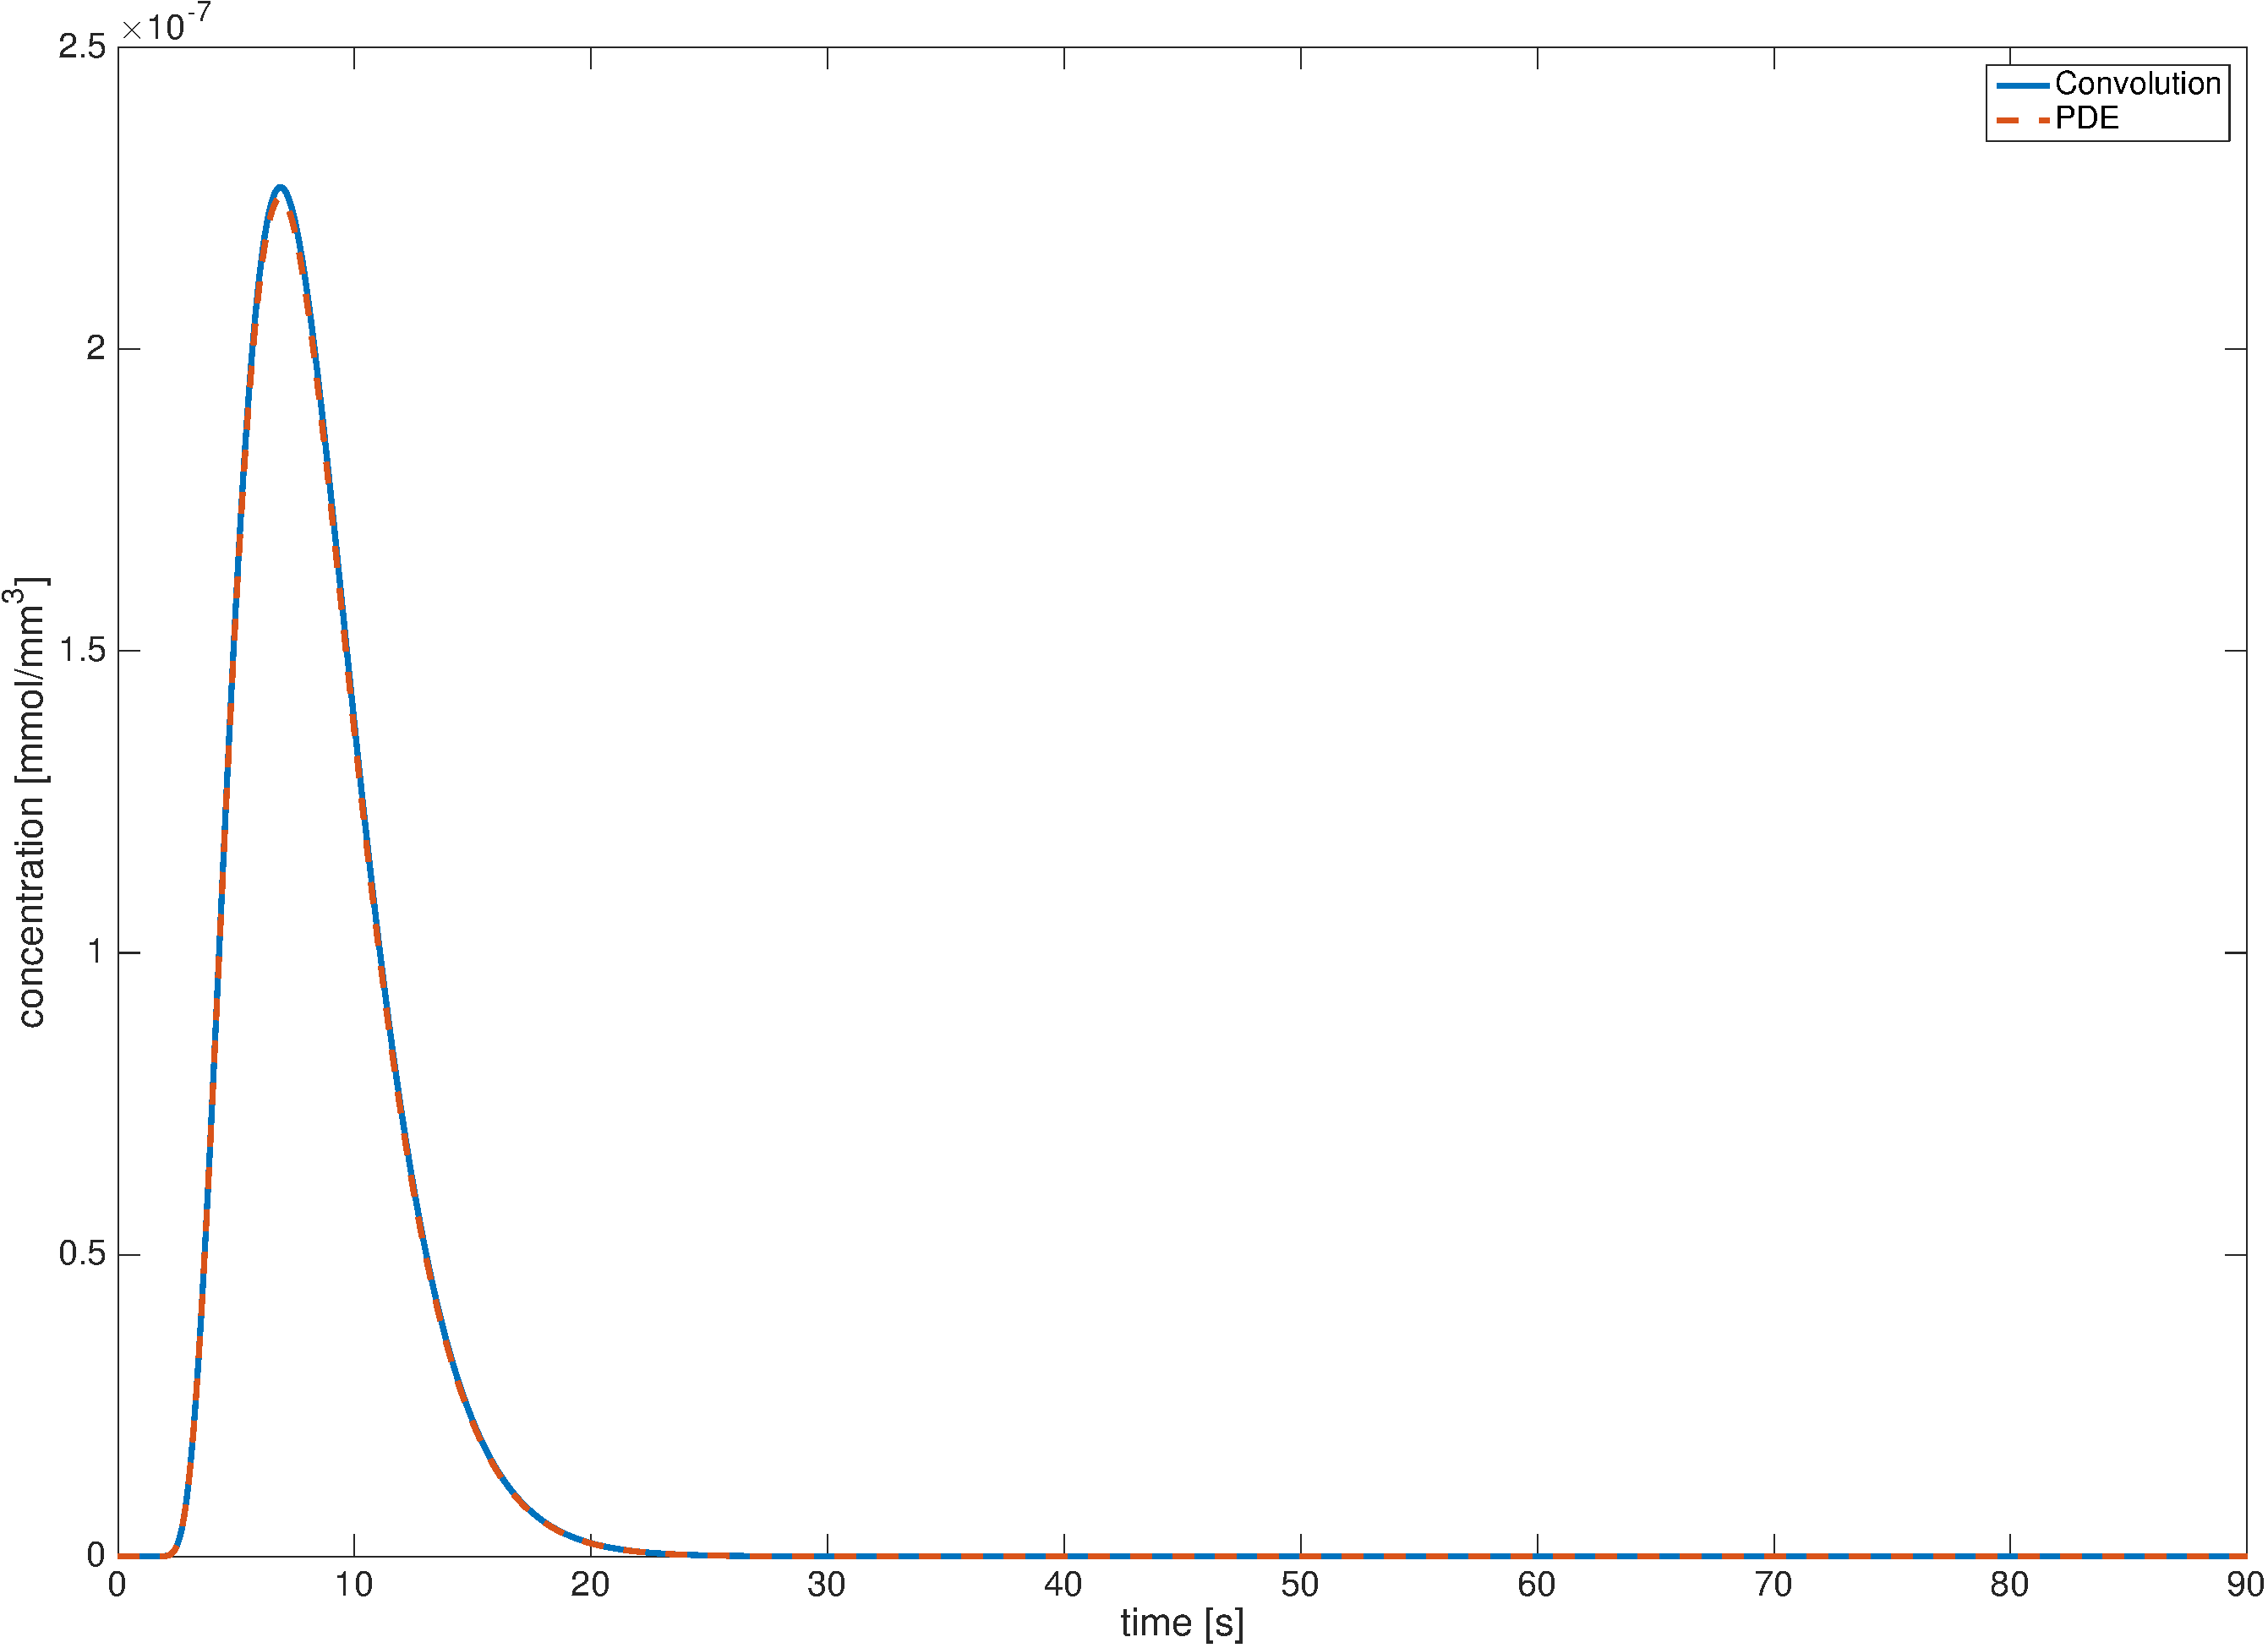
\includegraphics[width=\fwd]{./figs/ConvVsPDE.pdf} & 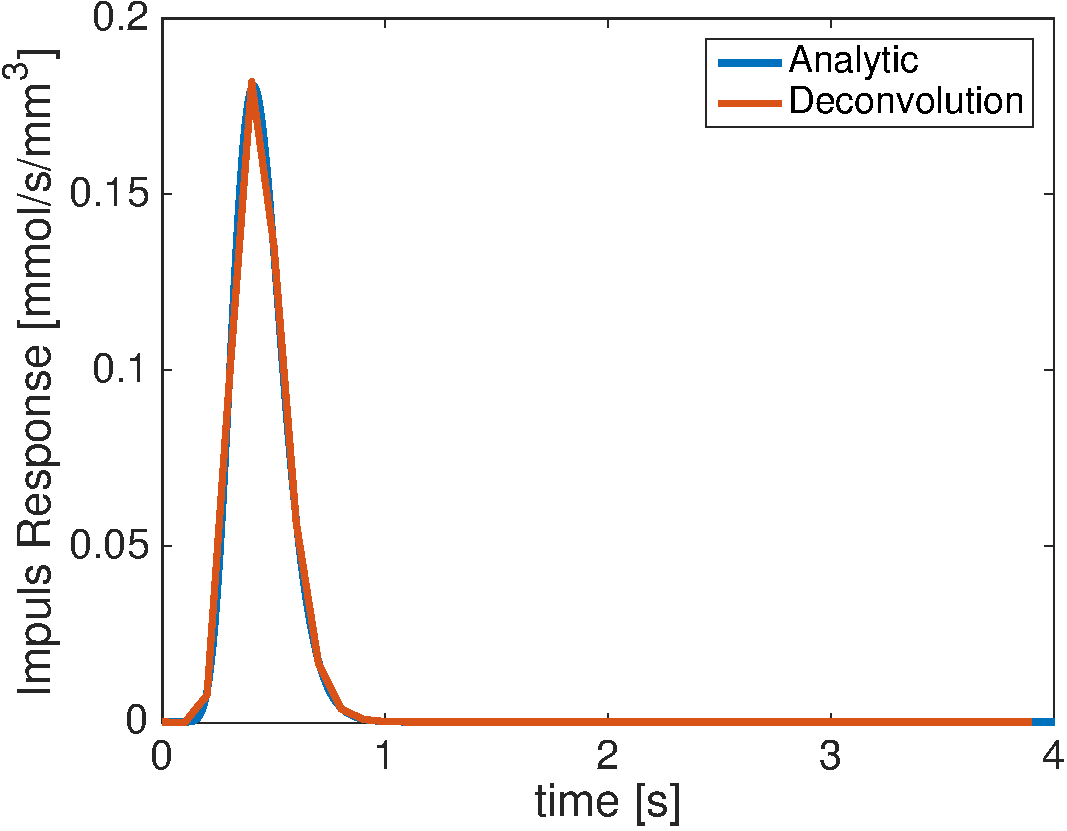
\includegraphics[width=\fwd]{./figs/IDecVsIAna.pdf} \\
		\end{tabular}
		\caption{Left: Red curve shows the tissue curve of the continuous PDE model at location [32,35]. Blue curve shows simulation using \eqref{eq:voxelcurve} with $P_i=\SI{5328}{\siPml}$ and $c_{\mathrm{in}}$ taken locally from upstream voxels around the simulated voxel. The two curves have an almost perfect overlap. Note that the perfusion is unrealisticly high since normalization is performed with respect to the volume of only one voxel. Right: Red curve shows the numerical impulse response functions at location [1,20] using the global arterial input function. Blue curve shows the analytic impulse response function given by \eqref{eq:IAna}. The two curves have an almost perfect overlap. These numerical experiments support the analytic considerations, that the computed impulse response function by traditional methods is not the directly feeding impulse response function, but rather a recursive impulse response function depending on all upstream voxels. }\label{fig:VoxelComp}
	\end{figure}
	

	%--------------------------------------------------
	% Subsection: Converting Flow to Perfusion
	%--------------------------------------------------
	\subsection{Converting Flow to Perfusion}\label{sec:flux2perf}
	The model described in \eqref{eq:flowmodel} uniquely determines the flux field $q(x)$. 
	However, in pharmacokinetic modeling the parameter of interest is usually the CBF, which we will denote by $\Perf (x)$ as the voxel wise field of perfusion. The surface flux and perfusion are physically distinct, and there are at least two differences between $q(x)$ and $\Perf (x)$. 
	First, the flux is a vector field and the perfusion is a scalar field. 
	Second, the flux is normalized to a surface area and the perfusion is normalized to a volume. 
	Thus, the surface flux and the perfusion are strictly, mathematically different but still conceptually related. 
	In the following we describe a method for converting flux into perfusion, motivated by our need to compare the ground-truth flux field to the scalar valued perfusion field obtained by traditional methods.

	The common understanding of perfusion or volume flux $\Perf (x)$ is the amount of blood feeding a tissue volume per unit time, with units [\si{\siQmm}]. 
	One straightforward approach for converting flux into perfusion could be to estimate the perfusion as the total inflow (or outflow) of fluid (e.g. arterial blood) into a control region per unit time, and then normalizing with the control region volume. 
	This is a valid approach only if the control regions are not feeding each other, and is therefore well-founded for the entire organ. 
	Such understanding of perfusion is in line with the theoretical foundation of traditional compartment models for perfusion where a control region has its own source of feeding arterial blood, independent of neighbor regions. 
	
	On the other hand, if the control region is a single voxel or a sub-division of an organ with sequentially feeding arterial blood, the traditional model assumptions are violated since every control region will feed its neighbours, thus becoming a coupled system of flow. 
	Simply summing the total inflow into a voxel and dividing by the voxel volume will strongly over-estimate the perfusion as the normalization refers to the wrong volume. 
	This phenomenon is demonstrated in Fig. \ref{fig:perfusion-problem} where the volume on the left has the true perfusion of $\Perf_{1} = \Flow_0 /(2V)$ for an incoming flow $\Flow_0$ [$\si{\siFmm}$] and distribution volume $2V$ [$\si{\simm}$]. 
	However, for another discretization as shown in the middle, the perfusion within each of these sub-volumes becomes $\Perf_{2} = F_0/V = 2\Perf_{1}$. 
	Taking the average across the two sub-volumes, it is clear that the perfusion is over-estimated with a factor of two. 
	A discretization dependent perfusion estimate is not recommendable, and the perfusion estimate of $\Perf_{2}$ is clearly wrong. 

	\begin{figure}[h!tb]
	    \centering
	    \begin{overpic}[scale=0.3]{figs/perfusion-problem.eps}
	    	\put(11,70){\color{black}$F_0$}
			\put(49,70){\color{black}$F_0$}
			\put(85.0,70){\color{black}$\Delta F_0$}
			\put(13,33){\color{black}$2V$}
			\put(50,20){\color{black}$V$}
			\put(50,45){\color{black}$V$}
			\put(91,42){\color{black}$\Delta V$}
		\end{overpic}
	    \caption{Perfusion within a small volume. Left: A compartment with volume $2V$ is exposed to a flow $\Flow_0$ [$\si{\siFmm}$] of fluid. By definition, the perfusion within this compartment becomes $\Perf_{1} = \Flow_0/(2V)$. Middle: The same volume is divided into two compartments (e.g. voxels), and the perfusion for each of the compartments becomes $\Perf_{2} = \Flow_0/V = 2\Perf_{1}$. The discrepancy between the two discretizations occurs because the flow is counted twice as it is fed from one voxel to the other. Right: As a solution to the described problem we rather pick out a true distribution volume $\Delta V$ (area in this 2D sketch), which is a small area around a given streamline along the centre line of the grey area. This is the true distribution volume (area in this 2D sketch) which is fed with arterial blood from the incoming fractional flow $\Delta \Flow_0$. The correct perfusion within $\Delta V$ is therefore $\Delta F_0/\Delta V$. The entire compartment can further be divided into similar infinitesimal distribution volumes, thus providing locally correct perfusion estimates.}
	    \label{fig:perfusion-problem}
	\end{figure}

	In the following we introduce a meaningful notion of perfusion for the continuous model.
	To do this, we will consider distribution volumes which are following the streamlines.
	For each point of a streamline we will select a small perpendicular disk with radius chosen in such a way that the total flow over each disk is constant along the streamline.
	% This disks will form a small tube around the streamline with constant flow over each cross-section.
	%Since the total flow over each disk is constant, we can define the perfusion for each voxel by the traditional model, obtaining a perfusion value which is constant along the streamline.
	%To obtain a truly local perfusion, we will let the radii of the disks go to zero.
	
	More precisely, let us consider an arbitrary streamline $S \subseteq \Omega \subseteq \R^3$ of length $l>0$ and parametrization $s:[0,l] \to \Omega$.
	We start by calculating the total flow over a small 2-D disk which is perpendicular to the streamline.
	Let $y \in S$ be an arbitrary location along the streamline. 
	The total flow over a 2-D disk $B_r(y)$ perpendicular to the flow-field $q(y)$ is given by
	\[
		F(y,r) = \int_{B_r(y)} q(x) \cdot \nu \diffint A \text{ where }\nu := q(y)/\vert q(y) \vert.
	\]
	In order to calculate the perfusion, we need to establish the volume of a small tube around the streamline.
	We will not consider a tube with constant radius, but one with spatially varying radii $p:S \to \R^+$.
	The total volume of such a tube surrounding the streamline is given by
	\[
		V(p) = \int_0^l \pi (p(s))^2 \diffint s
	\]
	We define the perfusion at an arbitrary point $y \in S$ by
	\[
		P(y):=\lim_{\varepsilon \to 0} \frac{F(y,\varepsilon p(y))}{V(\varepsilon p)} \text{ for } p(x):=1/\sqrt{\vert q(x) \vert}.
	\]
	Note that the radii $p(x)$ are chosen in such a way that in the limit $\varepsilon \to 0$ the total flow is constant along the streamline. 
	To see this, let us assume that $q$ is differentiable with Jacobian $J$.
	Using a Taylor expansion of $q(x)$ around $y$ as well as a change of coordinates yields 
	% \begin{align*}
	% 	F(y,\varepsilon r)&=\int_{B_{\varepsilon r}(y)} \nu^\top q(x) \diffint x \\
	% 	&= \int_{B_{\varepsilon r}(y)} \nu^\top q(y)  + \nu^\top J(\xi) (x-y) \diffint x \\
	% 	&= \varepsilon^2 \pi  + \int_{B_{1}(0)} \nu^\top J(\zeta) \varepsilon^3 \diffint x \\
	% 	&= \varepsilon^2 \left(\pi + \varepsilon \int_{B_{1}(0)} \nu^\top J(\zeta) \diffint x\right)
	% \end{align*}
	\[
		F(y,\varepsilon r)
		= \varepsilon^2 \Big(\pi + \varepsilon \int_{B_{1}(0)} \nu^\top J(\zeta) \diffint x\Big)
	\]
	where $\zeta \in (0,x)$ and simplifications are due to $r = p(y) = 1/\sqrt{\vert q(y)} \vert$ and $\nu:=q(y)/\vert q(y) \vert$.
	Note that since $V(\varepsilon p) = \varepsilon^2 V(p)$ it follows that
	\begin{equation}\label{eq:flux2perf}
		P(y)= \frac{\pi}{V(p)}
	\end{equation}
	Equation \eqref{eq:flux2perf} is independent of the spatial location $y$ along the streamline and an explicit formula for converting flux into perfusion, showing that a volume flux like perfusion scales with the distribution volume $V(p)$, which is a function of the streamline length.
	

	%--------------------------------------------------
	% Subsection: Estimate the Porosity
	%--------------------------------------------------	
	\subsection{A Method to Estimate local Porosity}\label{sec:CBV}
	
	It is known from literature on traditional models for perfusion that CBV for the entire compartment can be expressed as
	\begin{equation}
		\phi = \frac{\int_0^\infty C(t) dt}{\int_0^\infty c_a(t) dt}.
		\label{eq:CBV}
	\end{equation}
	where $C(t)$ are the tracer concentration with respect to a well mixed compartment and $c_a(t)$ is the tracer plasma concentration of the arterial input.
	However, it is not obvious that \eqref{eq:CBV} is valid also for a continuous one-compartment field model where the voxels are feeding each other. We will now proof that \eqref{eq:CBV} is nevertheless valid.
	
	Returning to the local definition of fluid tracer concentration as $c(x,t)$, the PDE in \eqref{eq:conteqlocal} is consistent with
	\begin{equation}
		\phi\frac{\partial c}{\partial t}  = - q \cdot \nabla c.
		\label{eq:1cmodel}
	\end{equation}
	for locations $x$ where $Q(x) = 0$.
	Integrating from $t_0$ to $t_1$ results in the model
	\begin{equation}
		\phi [c(x,t_1) - c(x,t_0)]  = - \int_{t_0}^{t_1}q \cdot  \nabla c \diffint t.
	\end{equation}
	Approaching the limit $t_0 = 0, t_1 = \infty$, using the boundary conditions $c(x,0) = c(x,\infty) = 0$ and defining $E(x):= \int_0^\infty c(x,t) \diffint t$ leads to
	\begin{equation}
		0 = q \cdot \nabla  E(x).
		\label{eq:streamlinezero}
	\end{equation}
	We can interpret this equation such that $q$ is tangent to the level-sets of the function $E(x)$, which means that $E(x)$ is constant along the streamlines of the fluid flow.
	Since at the beginning of the streamline it holds by construction that $c(x_0,t) = \ca(t)$ and since $C(x,t) = \phi(x) c(x,t)$ it follows that 	
	\begin{equation}
		\phi(x) =  \frac{ \int_{0}^{\infty} C(x,t) \diffint t }{\int_{0}^{\infty} \ca(t) \diffint t}.
		\label{eq:phi}
	\end{equation}
	Note that equation \eqref{eq:phi} coincides with the traditional formula \eqref{eq:CBV} for $\phi$.
	
	
	%--------------------------------------------------
	%--------------------------------------------------
	% Section: Experiments
	%--------------------------------------------------
	%--------------------------------------------------
	\section{Numerical Experiments}\label{sec:NumExp}
Based on the field models described in Section \ref{sec:synthetic}, we now establish an experimental setup suited to study the performance of the traditional methods in a synthetic flow field with a known ground truth.

	Based on \eqref{eq:flowmodel} and \eqref{eq:conteqlocal} we set up a forward simulation of blood-flow and indicator dilution through the capillary system. The source can be understood as the arterial space, and the sink can be understood as the venous space. We aimed at creating a transparent synthetic test case and kept all optional parameters as simple as possible. 
	
	We chose a standard arterial input function \cite{ostergaard96}, the gamma-variate function
	\begin{equation}
		\ca(t) := D_0(t-t_0)^\alpha e^{-(t-t_0)/\beta}
	\end{equation}
	for default parameters $\alpha=3$, $D_0 = 1$, $\beta = \SI{1.5}{\second}$ and $t_0 = \SI{0}{\second}$.
	Ground truth perfusion for the domain of size $\SI{3}{\milli\meter}\times\SI{3}{\milli\meter}\times\SI{1}{\milli\meter}$ was chosen $50$\si{\siPml}.
	The source term was assigned to the upper left voxel and the sink term was assigned to the lower right voxel.
	It was assumed that both the domain of inflow as well as outflow were approximately of the voxel-size, leading numerically to Delta-like source and sink terms $\Qso$ and $\Qsi$.
	Permeability was chosen isotropic and constant throughout the domain $\mathbf{k}=\SI{5e-6}{\square\milli\meter}$, assuming no directional bias of the capillary system.
	Dynamic blood viscosity was chosen $\mu=\SI{5e-6}{\simu}$ according to \cite{rosencranz06}.
	Porosity (e.g. CBV) was assumed to be $\phi = 0.05$.
	Since our aim was to test limits of established methods and to simulate high resolution scans, a voxel size of $(\SI{0.05}{\milli\meter},\SI{0.05}{\milli\meter},\SI{3}{\milli\meter})$ was assumed.
	The flow field is visualized in Figure \ref{fig:flowpressureperfusion} (a).
	% is vector flux integrated across cell surface, $\int_{\partial \Omega_{ij}}q \diffint s$.
	%  with units [\si{\siFmm}].
	
	Equation \eqref{eq:flowmodel} was solved numerically using two-point flux-approximation (TPFA) widely used in reservoir mechanics \cite{Aarnes2007}.
	The transport described in \eqref{eq:conteq} was implemented using first order upwinding \cite{Patankar80}, yielding a 4D CA concentration map $C(x_i,t_j)$.
	From the porous media model using \eqref{eq:flowmodel} and \eqref{eq:conteqlocal}, streamlines were found from tracking of the flux vector field $q$ by FACT \cite{Mori1998}, known from  tractography within diffusion tensor imaging (DTI). 
	
\begin{figure*}[h!tb]
	\centering
	\begin{tabular}{c c c}
		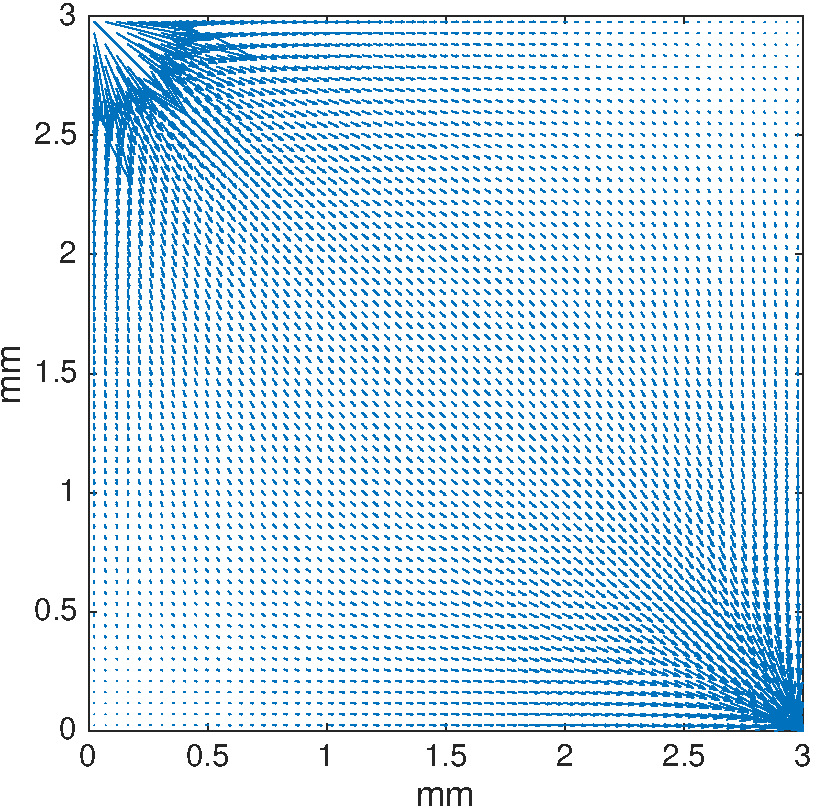
\includegraphics[width=.3\textwidth]{figs/qmat.pdf} & 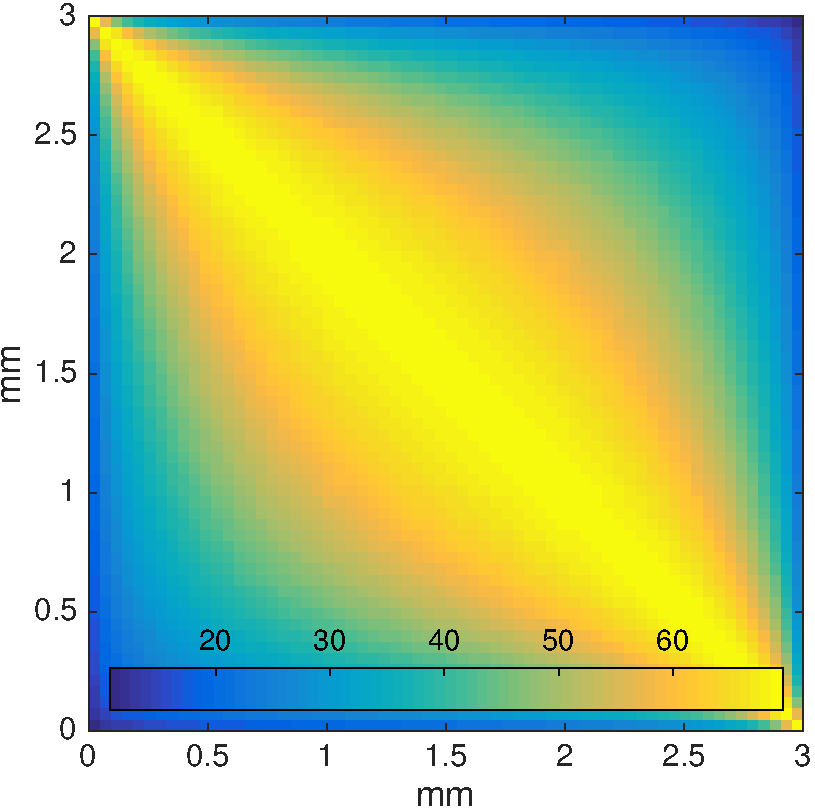
\includegraphics[width=.3\textwidth]{figs/perfmat.pdf} & 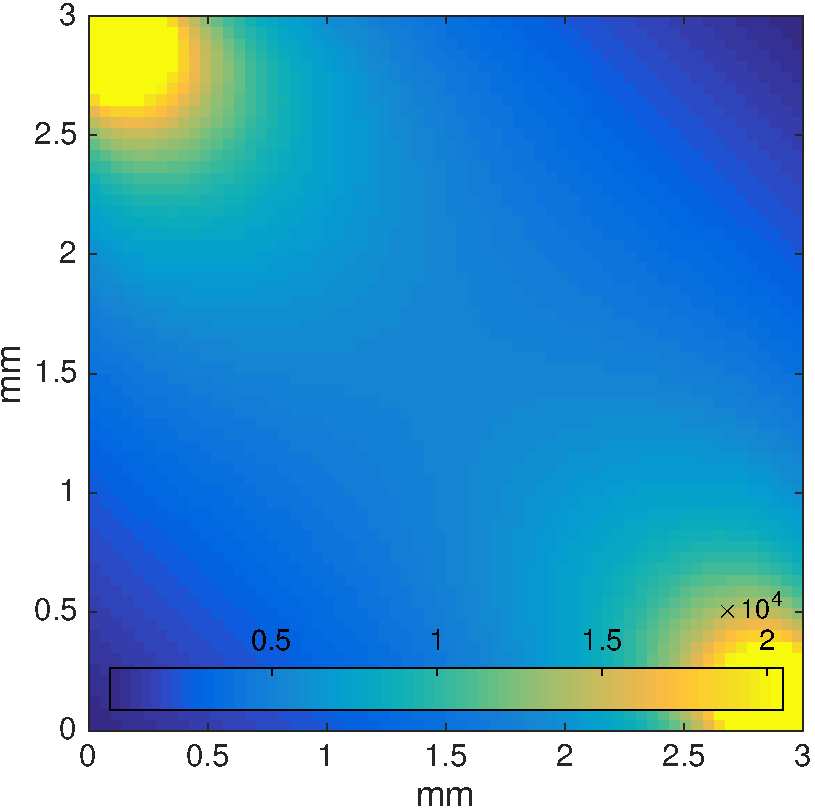
\includegraphics[width=.3\textwidth]{figs/lperfmat.pdf}\\
		(a) Flow field & (b) Perfusion $\Perfs$ along the streamlines  & (c) Local perfusion $\Perfv$.
	\end{tabular}
	\caption{Porous media (PM) flow model with a source in the upper left corner and a sink in the lower right corner. (a) Flow field used to simulate distribution of the contrast agent, (b) Perfusion along the streamlines according to \eqref{eq:flux2perf}, (c) Local perfusion according to \eqref{eq:perflocal}.}
        \label{fig:flowpressureperfusion}
\end{figure*}


%	%--------------------------------------------------
%	%--------------------------------------------------
%	% Section: Results
%	%--------------------------------------------------
%	%--------------------------------------------------
	\section{Results}	
	\subsection{Reconstruction of perfusion within synthetic data}\label{sec:RecPhantom}


	We tested the convolution based traditional model (bSVD) \eqref{eq:conv} as well as maximum-slope (MS) model \eqref{eq:MS} for their capability to recover perfusion.
	Prior to reconstruction, the CA concentration map $C(x,t)$ was downsampled to a time-resolution of $\SI{.2}{\second}$ in order to stay within comparable time sampling existing on modern MR equipment for dynamic imaging.
	In order to simulate different spatial resolutions of the scanning process, the data was averaged using different block-sizes ranging from $(1,1)$ pixel to $(64,64)$ pixels.		
	Success of restoration was measured in terms of the relative error of the recovered perfusion with respect to the ground truth perfusion, $RE := \vert \Perf_{\mathrm{rec}} - \Perf_{\mathrm{true}}/\Perf_{\mathrm{true}}\cdot 100\%$.
	The recovered perfusion was compared against the two perfusion maps depicted in Figure~\ref{fig:flowpressureperfusion}:
	
	The local perfusion map $\Perfv$ was set up using the local definition definition \eqref{eq:perflocal}. 
	Since normalization is performed with respect to voxel size, the values are unrealistically high and will vary with the discretization.
	As equation \eqref{eq:voxelcurve} shows, this can nevertheless be regarded a valid definition of perfusion since it models the feeding of arterial blood to a control region.
	To quantify the errors occurring by traditional methods, the global arterial input function was used for the deconvolution, cf. \eqref{eq:IAna}.
	% Since the corresponding impulse response functions are decaying rapidly, this makes the deconvolution especially sensitive to downsampling of the time-curves..

	The global perfusion map $\Perfs$ was set up using the definition along the streamlines \eqref{eq:flux2perf}.
	This definition most accurately reflects the physical perfusion at a given location and shows plausible perfusion values, cf. Figure~\ref{fig:flowpressureperfusion}.
	However, we do not expect the traditional models to be able to recover these values accurately.
	% Errors are given to indicate the amount of overestimation by standard methods.
	
	Results are displayed in Table \ref{tab:resultsSim}. 
	For the complete system, both the maximum slope method and the convolution method could restore the ground truth perfusion of \SI{50}{\siPml} accurately with errors of $<1\%$ and $4\%$ respectively.
	However, this changes if the methods are applied only to parts of the system.
	If compared to $\Perfv$, one can see that results are clearly improving with increasing block size. Note that the block size of $(0.5,0.5)\SI{}{\milli\meter}$ is within the range of resolution available on clinical scanners today, and is therefore clinically interesting.
	Also a clear advantage of the bSVD method as compared to MS can be observed.
	This is possibly to the additional assumptions of the MS method.
	If compared to $\Perfs$, rendering both methods incapable to recover the physically more meaningful notion of perfusion along the streamlines.
		
	Results from reconstructing $\phi$ are shown in also shown in Table~\ref{tab:resultsSim}, where the relative errors are low for both forward data generated by the transport equation as well as the convolution model.
	This is supported by the analytic considerations in Section~\ref{sec:CBV}.
	
	\begin{table}[h!tb]
		\scriptsize
		\caption{Relative error $RE$ (\%) for reconstructing perfusion $\Perfv$, $\Perfs$ and the blood volume $\phi$. Displayed is the median $RE$. Both reconstruction models MS and bSVD are able to restore the perfusion for the entire domain, but fail when dividing the domain into smaller block sizes. For larger block-sizes the bSVD model restores the perfusion more accurately than the MS model. However, the blood volume $\phi$ is recovered accurately. Note that voxel size $(0.05,0.05)$ corresponds to the original voxel size (block size of (1,1) voxels) in the PDE model. For a more detailed discussion see Section~\ref{sec:RecPhantom}.}
		\centering
		\begin{tabular}{p{1cm} c c c c c}
						& \multicolumn{2}{c}{$\Perfv$} & CBV & \multicolumn{2}{c}{$\Perfs$}  \\
			voxel size (mm)	& bSVD	& MS 	&  		& bSVD	& MS 	\\ \toprule
			(0.05,0.05) 		& 93\%	& 98\%  & <1\%  & 423\%	& 95\% 	\\
			(0.23,0.23) 		& 67\%	& 90\% 	& <1\% 	& 387\%	& 90\% 	\\
			(0.5,0.5) 	& 44\%	& 79\% 	& <1\% 	& 292\%	& 82\% 	\\
			full domain   	& 4\%	& <1\%  & <1\%	& 		& 	   
		\end{tabular}
		\label{tab:resultsSim}
	\end{table}
	
	
	%--------------------------------------------------
	%--------------------------------------------------
	% Subsection: Results on Real Data
	%--------------------------------------------------
	%--------------------------------------------------	
	\subsection{Reconstruction of perfusion within real data}\label{sec:RealData}
 	Experimental results from Section \ref{sec:RecPhantom} indicate that application of the deconvolution model to patches of tissues violating the model assumptions would lead to overestimation of blood-flow as compared to the overall flow within the volume of interest.
	In order to validate this guess, we applied the deconvolution model to a clinically acquired human perfusion CT dataset of a 56 years old male male admitted with suspicion of stroke to the Radboud University Medical Center in Nijmegen, the Netherlands.
	The perfusion scan was obtained using a Toshiba Aquilon ONE scanner, pixel-size $\SI{0.43}{\milli\meter}\times\SI{0.43}{\milli\meter}$, slice thickness $\SI{0.5}{\milli\meter}$, contrast agent \SI{50}{\milli\liter} Xentix 300, total scan-time \SI{114}{\second}, time resolution ranging from \SI{2.1}{\second} in the early- to \SI{30}{\second} in the late phase of CA uptake.
	The arterial input function was manually selected by a medical expert within the middle cerebral artery (MCA).
	Since we expected to see local overestimation effects mainly for small voxel sizes, the data was processed at full resolution ($512\times512\times320$). 
	However, in order to deal with noise effects it was necessary to apply a prior gaussian smoothing with standard deviation of $1$ voxel.	
	Relative concentrations were estimated from the CT signal assuming a spatially independent proportionality constant.
	CBF was then estimated voxel-wise using a Matlab implementation of bSVD, yielding an average CBF of \SI{64.357}{\siPml}.
	After that, we estimated the perfusion for the whole volume of interest by averaging the concentration values first and then performing the bSVD, yielding a total CBF of \SI{24.791}{\siPml}.
	Results are depicted in Fig. \ref{fig:RealData}
	
	\begin{figure*}[h!tb]\label{fig:RealData}
		\begin{tabular}{p{.3\textwidth} p{.3\textwidth} p{.3\textwidth} }
		 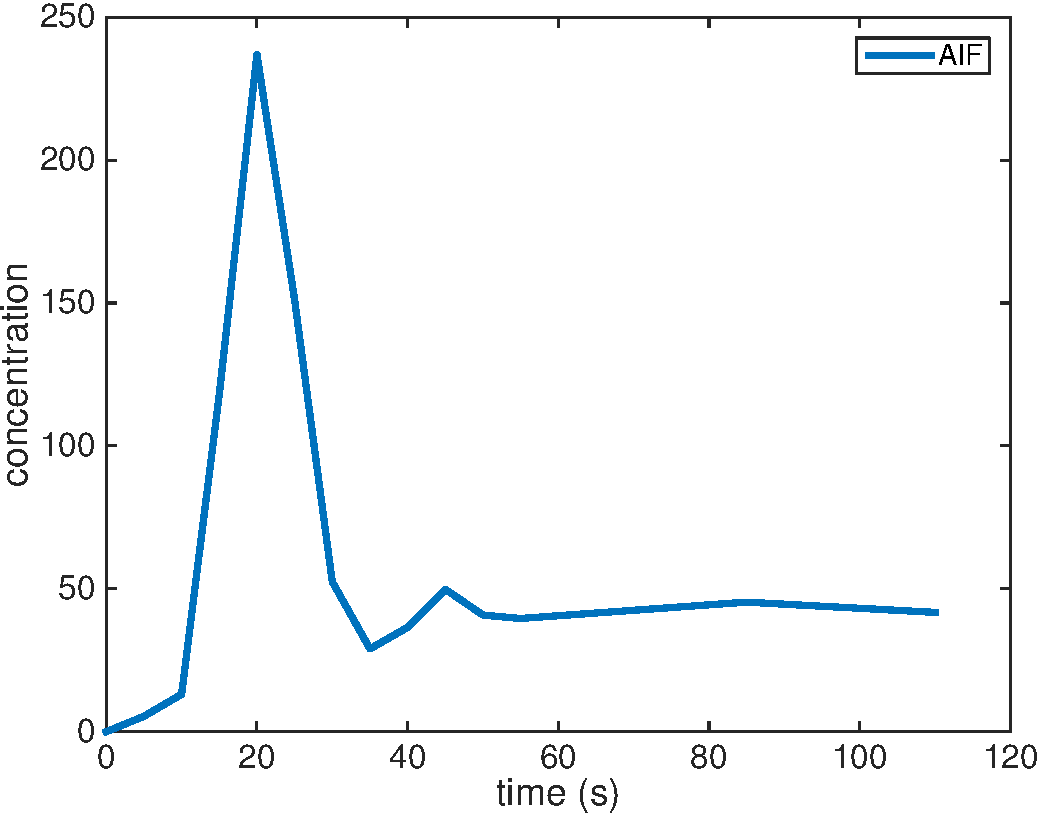
\includegraphics[width = .3\textwidth]{./figs/real_AIF.pdf} & 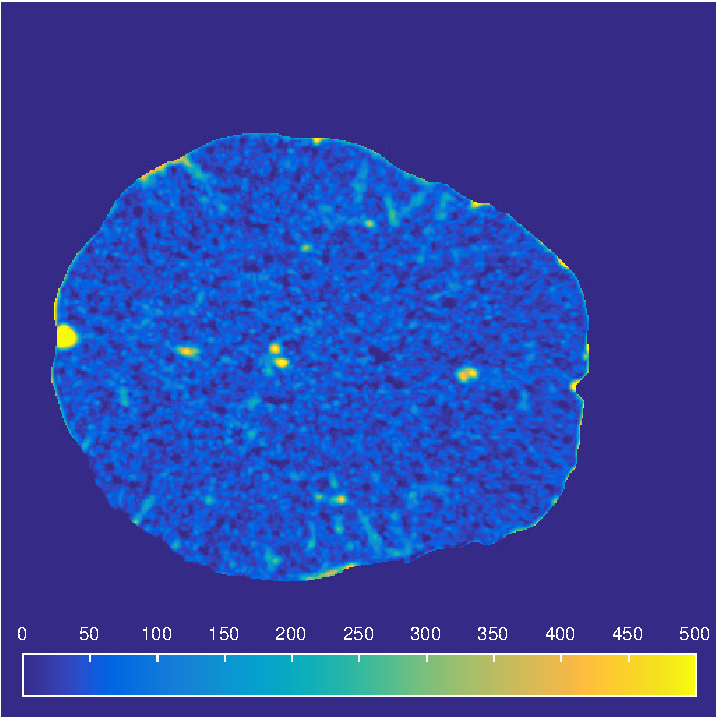
\includegraphics[width = .3\textwidth]{./figs/real_axial160.pdf} & 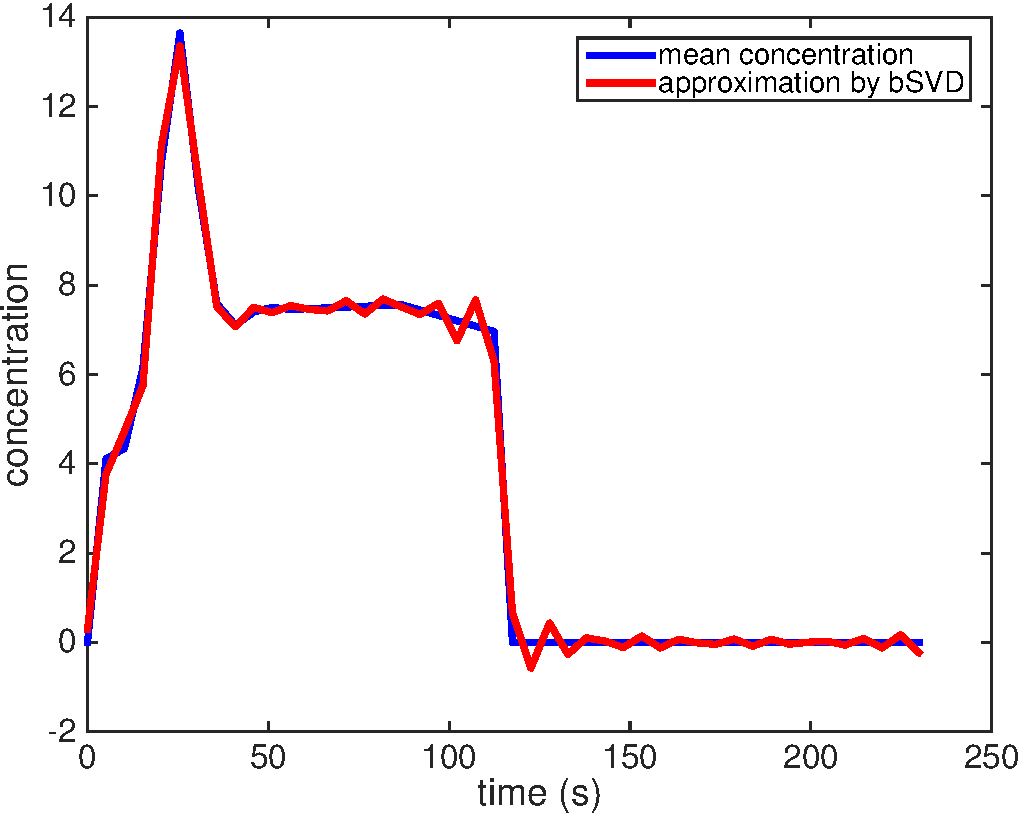
\includegraphics[width = .3\textwidth]{./figs/real_meanC.pdf} \\
		 (a) Arterial input function & (b) One slice of the voxel-wise CBF reconstruction.  & (c) Mean CA concentration curve of the whole volume of interest for reconstruction.
		\end{tabular}
		\caption{Figure with results from the real-data experiments (see Sec. \ref{sec:RealData} for details on the data). (a) AIF manually selected from the MCA. (b) One slice of the voxel-wise CBF-reconstruction for a 3D volume of interest. (c) Mean concentration curve for the complete 3D volume of interest and the curve approximation by bSVD.}
	\end{figure*}
	

	
	
	%--------------------------------------------------
	%--------------------------------------------------
	% Section: Discussion
	%--------------------------------------------------
	%--------------------------------------------------	
	\section{Discussion}\label{sec:conclusion}
	
	In this work we have studied the impact of traditional models to perfusion reconstruction in a coupled system of 1C models.
	To establish ground-truth values, we developed a PDE based digital phantom to simulate blood flow within a slab of tissue with a highly developed capillary system.
	We have shown that the discretized PDE problem can be equivalently described as a system of coupled traditional one-compartment models.
	
	
	
	
	The results strongly support the usage of traditional models for entire regions which are fed directly by the measured arterial input.
	They also show show that if traditional models are applied only to parts of the system, they tend to overestimate the actual perfusion. The reason for this is that traditional models do not take into account the correct distribution volume of the feeding arterial flow.
	Note that taking local arterial input functions is no remedy for this problem, since the resulting perfusion will depend heavily on the voxel size and overestimate the actual flow, cf. Figure~\ref{fig:perfusion-problem} and \eqref{eq:voxelcurve}.
	In fact, in the most extreme example we measured overestimated perfusion values of up to $423\%$.
	The results from the digital phantom are supported by real-data experiments, where we showed local overestimation of perfusion for small voxel-sizes as compared to an averaging of concentrations for the entire volume of interest.
	Regarding the CBV estimates, one can observe from Table \ref{tab:resultsSim} that estimation of blood volume is far more stable, and  
	even various block sizes had little impact on the results. 
	These results are in well agreement with the analytical observations described in Section \ref{sec:CBV}, stating that \eqref{eq:CBV} is valid for entire organs as well as for single voxels. 
	Thus, these results support the usage of \eqref{eq:CBV} for computing the CBV with high accuracy for any type of block size, including single voxels.



	Furthermore we have introduced two conceptually interesting mathematical definitions of voxel perfusion.
	The global perfusion $\Perfs$ models perfusion along the streamlines and most accurately models the physical notion of volume flow within the correct distribution volume.
	Theory and experiments show that the traditional models cannot recover this perfusion. The usage of $\Perfs$ in reconstructing perfusion might as well be challenging as the entire geometry and microscopical flow patterns would have to be known to track the streamlines. However, for our purpose the understanding of perfusion as a blood flow that must be normalized along its entire length from transition of arterial to venous blood, was useful. On the other hand, for future developments of field models for reconstructing perfusion, multi compartment models as suggested in \cite{sourbron14} might be more applicable.
	
	Perfusion $\Perfv$ was set up based on the interpretation of a coupled system between adjacent voxels. However, this estimate for perfusion will be over-estimated and was only useful within the computations we performed.
	Theory and examples show that this definition does not comply with the intended physical notion since it depends heavily on the discretization.
	However, we have shown that traditional models would restore this value if the correct (local) arterial input function was selected.
	We have additionally analyzed the impact of selecting a further upstream arterial input function both analytically and experimentally.
	Specifically we have given an analytic expression which shows that the perfusion will depend on the flow at all upstream voxels, and that the traditional convolution method actually finds the recursive impule response function for all upstream voxels according to \eqref{eq:IAna}.
	
	In conclusion, our experiments show that the traditional methods for perfusion estimation perform well when applied to the entire domain, but they tend to fail when applied to smaller block sizes positioned downstream in the flow. The reason for this failure is not numerical instabilities in the deconvolution, but rather over-simplification of a physical phenomenon that is inter-connected in space.  The perfusion becomes over estimated as the traditional models will not account for the streamline length of the flow in the transition phase when becoming venous blood, and the same flow will be counted multiple times. This problem is expected to become more pronounced in future as imaging hardware is constantly improving in spatial resolution, yielding high resolution images of sub-millimeter accuracy where a capillary patch with a common arterial input becomes separated between neighboring voxels. 
	To account for this problem, the development of new field models for perfusion is therefore highly demanded, in line with approaches described in \cite{sourbron14,Michler2013}. 	
	
	% Experiments show, that estimations results improve if block-sizes are increasing.
	% Estimation of CBV however has been shown to be stable.
	
	%Our results indicate the traditional models should only be used for larger computational units where the arterial input is an actual arterial input for the domain as a whole. 


	
	%--------------------------------------------------
	% Bibliography
	%--------------------------------------------------
	\bibliographystyle{IEEEtran}	
	\bibliography{./bibliography}
	

\end{document}